\begin{titlepage}

% Logos

\includegraphics[width=200px]{./images/logo-hsr}
\hfill
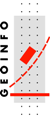
\includegraphics[width=40px]{./images/logo-geoinfo}
\vspace{2.2cm}

\begin{center}
{ \Large
	% Titel
	\textbf{Cloudbasiertes Geodatenmanagement mit Google Fusion Tables: Entwicklung eines Cloud-GIS Prototypen}
	\vspace{1cm}

	% Arbeitstyp / Schule
	\textbf{Studienarbeit}
	\vspace{1cm}

	Abteilung Informatik \\[0.2cm]
	Hochschule für Technik Rapperswil
	\vspace{1cm}

	% Semester
	Frühjahrssemester 2012
}
\end{center}
\vspace{2.3cm}

\begin{tabular}{p{0.19\twocelltabwidth}p{0.81\twocelltabwidth}}
Autoren: & \textbf{Stefan Oderbolz} (\url{soderbol@hsr.ch}) \newline
 \textbf{Jürg Hunziker} (\url{jhunzike@hsr.ch}) \\ 
Betreuer: & \textbf{Prof. Stefan Keller} (\url{sfkeller@hsr.ch}) \\ 
Projektpartner: & \textbf{Marco Lehmann}, GEOINFO AG Herisau, \url{http://www.geoinfo.ch} \\ 
Experte: & \textbf{Prof. Stefan Keller} (\url{sfkeller@hsr.ch}) \\ 
Datum: & \textbf{29. Mai 2012} \\ 
\end{tabular}

\end{titlepage}